\documentclass[memoire.tex]{subfiles}

\chapter{Classement supervisé}
\section{Introduction}
Il existe de nombreuses méthodes de classement supervisé. L'objectif est d'analyse les algorithmes les plus importants et utilisés afin de mettre en avant la partie mise en œuvre de l'apprentissage supervisé et de comprendre le fonctionnement de chacun. La première méthode est le \textit{K-Nearest Neighbors}, suivie de CART, puis de ID3 et C4.5 pour finir par A*.

\section{K Nearest Neighbors}
\subsection{Concept}
La méthode des k plus proches voisins (\textit{K-Nearest Neighbors ou K-NN} est une méthode paresseuse d'apprentissage supervisée. Elle peut s'utiliser de différente manière, l'une étant pour le classement. \textit{Le problème des K-NN est de créer une structure de données pour un ensemble d'objets qui, étant donné un objet $q$, son plus proche voisin dans l'ensemble peut être trouver rapidement}.~\cite{knn} L'objectif est de placer les observations du jeu d'apprentissage sur un espace métrique. Naturellement, ces observations seront majoritairement regroupés vers un même espace. Lors de l'ajout d'une nouvelle instance, l'algorithme va analyser quels sont ses $k$ voisins les plus proches afin de déterminer la classe à attribuer. C'est un algorithme \textit{lazy} car celui-ci ne fait que très peu de traitement durant la phase d'apprentissage. Les calculs sont faits durant la phase de classement des données.\\

La figure 3.1 montre un ensemble de données\footnote{Disponible à l'adresse : \url{https://www.kaggle.com/alqamahjsr/topic-3-decision-trees-and-knn}} contenant deux attributs $x \in [0, 30]$ et $y \in [0, 30]$ et deux classes, l'une rouge et l'autre jaune. Il est clairement visible que les points rouges se trouvent sur la partie supérieure gauche du graphique tandis que les points jaunes, sur la partie inférieure droite (figure 3.2). Si une nouvelle instance apparaissait, $\forall k \in \mathbb{N}$, celle-ci serait relativement simple à classer.\\

En revanche, avec \textit{K-NN}, le choix du $k$ est arbitraire et celui-ci peut influencer le résultat obtenu.

\begin{figure}[!htb]
   \begin{minipage}{0.48\textwidth}
     \centering
     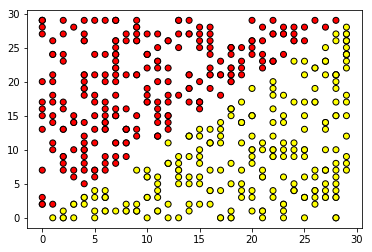
\includegraphics[width=.7\linewidth]{img/knn.png}
     \caption{Représentation graphique de points ayant pour classe "rouge" ou "jaune"}
   \end{minipage}\hfill
   \begin{minipage}{0.48\textwidth}
     \centering
     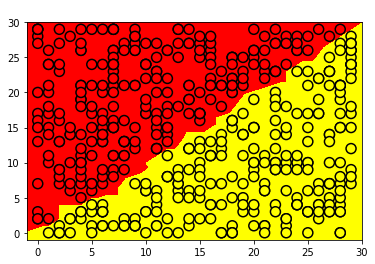
\includegraphics[width=.7\linewidth]{img/knn2.png}
     \caption{Séparation des données par leur classe}
   \end{minipage}
\end{figure}

\subsection{Choix de k}
$k$ est une valeur arbitraire choisie avant le lancement de l'algorithme. Cette valeur permet de choisir le nombre de voisins à regarder afin de déterminer la classe d'une observation. Cela signifie que si $k$ est trop petit, l'algorithme retournera la valeur de l'observation la plus proche. Un petit $k$ générera alors un modèle trop précis, qui engendrera un problème d'\textit{overfitting}. Dans le cas contraire, un trop grand $k$ pourrait réduire la précision du modèle et rendre le comportement du modèle trop abstrait~\cite{data_mining}.\\

Par exemple, la figure 3.3\footnote{Antti Ajanki AnAj - Own work, CC BY-SA 3.0, \url{https://commons.wikimedia.org/w/index.php?curid=2170282}} met en avant le problème du choix de $k$. Cette figure possède une observation de test (cercle vert) à classer soit en carré bleu, soit en triangle rouge. Dans le premier cas, $k = 3$, l'algorithme va donc regarder les trois voisins les plus proche du cercle : deux triangles rouges et un carré bleu et déduire que l'observation est un triangle rouge. Dans le deuxième cas, $k = 5$, les cinq plus proches voisins sont deux triangles rouges et trois triangles bleus : l'observation sera alors un carré bleu. Dans cet exemple, un $k$ trop grand a changer la classe en carré bleu alors que celle-ci semble être plus proche des triangles rouge.\\

\begin{figure}[!h]
	\centering
	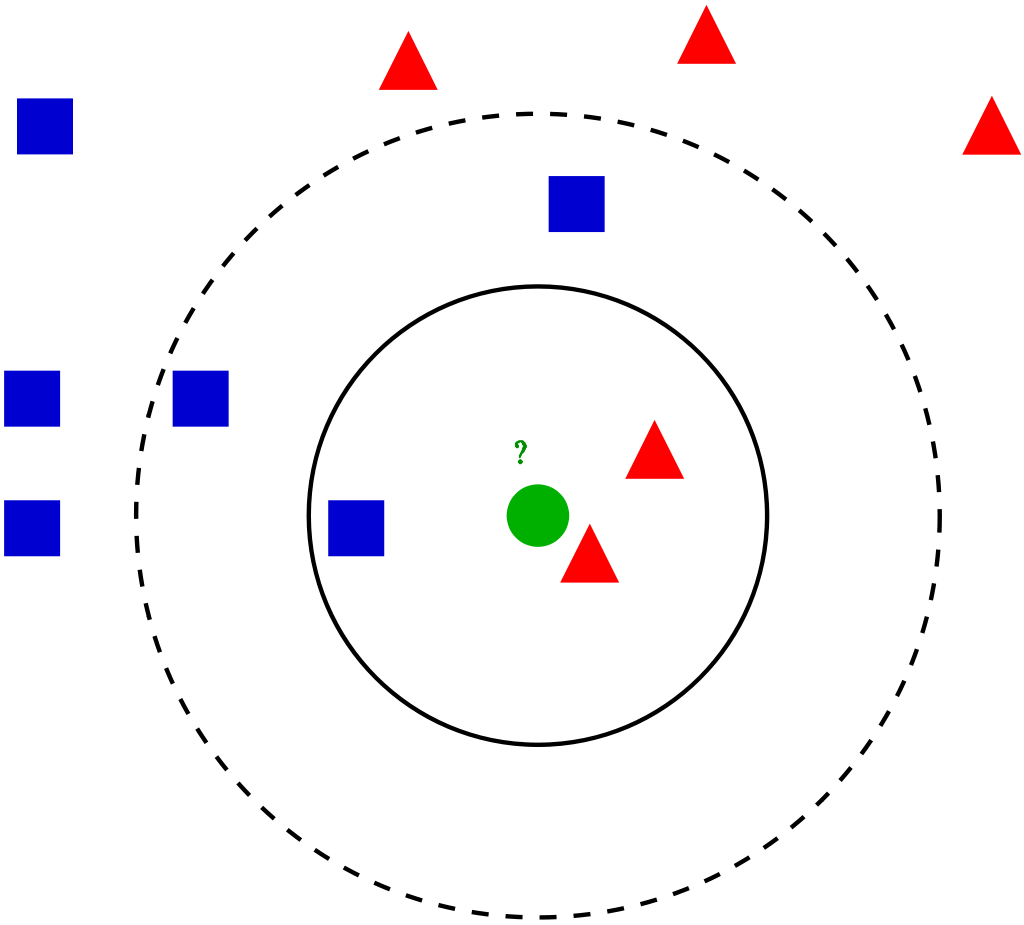
\includegraphics[scale=0.15]{img/knnk.png}
	\caption{Exemple de K-NN avec deux valeurs différentes de $k$}
\end{figure}

Afin d'améliorer \textit{K-NN}, il est possible de donner un poids aux voisins et aux attributs. Ainsi, un voisin proche aura plus d'importance qu'un voisin éloigné qui risque de ne pas être de la même classe. Par ailleurs, un attribut n'étant pas pertinent aura beaucoup moins d'importance qu'un attribut aidant au classement~\cite{data_mining}.


\section{CART}
\textit{Classification And Regression Trees} (CART) est une méthode développée par~\citeauthor{cart}~\cite{cart}. Cette approche permet de créer des arbres binaires (chaque nœud a deux descendants directs). Chaque test, ou \textit{split}, correspond à la question binaire qui maximise la réduction de l'entropie. Pour cela, l'algorithme va parcourir tous les attributs de chaque nœud et garder le meilleur pour en dégager le \textit{split} maximisant la réduction de l'entropie. Il va ensuite comparer les \textit{splits} pour garder le meilleur. L'algorithme 1 montre le procédé suivant le choix du split. Les données sont alors séparées en deux : d'un côté celle qui répondent "vrai" au test et "faux" de l'autre. Ces actions sont répétés autant de fois que nécessaire jusqu'à atteindre les feuilles de l'arbre ou un autre critère d'arrêt. 

\frame{
\begin{algorithm}[H]
 \KwData{jeu de données}
 \KwResult{arbre de décision}
  calcul du meilleur split et de son gain d'information\;
  \eIf{gain d'information = 0}{
   renvoie une feuille contenant les données\;
   }{
   récupérer les données "vraies" et "fausses" du split\;
   retour au début en donnant les données "vraies" comme paramètre\;
   retour au début en donnant les données "fausses" comme paramètre\;
  }

 \caption{Algorithme CART}
\end{algorithm}
}

Dans le cas où les attributs ne sont pas binaires, les questions posées sont alors de la forme :
\begin{itemize}
\item $x \leq 0.9$ ?
\item $v_1 \in V = \{v_1, v_2, v_n\}$, $\forall n \in \mathbb{N}$, $x = v_1$ ? 
\item $\forall i < n$, $x \in \{v_1, \dots, v_i\}$ ?
\end{itemize}
Chaque possibilité sera étudiée ce qui peut augmenter rapidement la complexité de l'algorithme si les nombres d'attributs ou de valeurs sont grands.

\section{C4.5}
C4.5 est un algorithme inventé par~\citeauthor{c4.5}~\cite{c4.5}. Comme pour CART, l'algorithme va parcourir chaque nœud récursivement et trouver le meilleur \textit{split} à chaque fois. Cependant, celui-ci ne se limite pas aux arbres binaires et peut donc avoir \textit{n} nœuds descendants. Pour des attributs qualitatifs, une branche sera créée pour chaque valeur possible. Pour choisir le meilleur \textit{split}, l'algorithme va utiliser le gain d'information (équation 1.13).\\

Une fois l'arbre construit, une fonction d'élagage (algorithme 2) est alors appelée afin d'améliorer les résultats. Cette méthode est appelée \textit{error-based pruning} est une amélioration du \textit{pessimistic pruning}~\cite{c4.5}. Selon Quinlan, $E$ objets mal classés sur $N$ observations amènent à un taux d'erreur optimiste de $\frac{E}{N}$. La borne supérieur $U_{CF}(E, N)$ de l'indice de confiance $CF$ peut être trouvée selon les limites de confiances de la distribution binomiale~\cite{c4.5}, ce qui correspond au taux d'erreur prédit pour une feuille. Ce niveau de confiance est une valeur donnée et vaut 25\%. Le but de l'algorithme est de comparer le taux d'erreur de chaque feuille avec les feuilles des sous-arbres correspondant. Si le taux d'erreur du sous-arbre (nœud parent) est inférieur à celui des feuilles, alors on élague le sous-arbre par une feuille.

\frame{
\begin{algorithm}[H]
 \KwData{E objets mal classés, N observations}
 \KwResult{arbre}
 \While{sous-arbres à parcourir}{
  erreur feuilles {$\leftarrow$} {$\sum_{}{} N \times U_{25}(E, N)$}\;
  erreur nœud parent {$\leftarrow$} {$N' \times U_{25}'(E', N')$}\;
  \eIf{erreur feuilles > erreur nœud parent}{
   nœud parent {$\leftarrow$} feuille\;
   }{nœud parent inchangé\;}
 }
 \caption{Élagage de l'algorithme C4.5}
\end{algorithm}
}